% Insert after the Airport sensitivity subsection; uses the same D1/D2 definitions.
\subsection{Sensitivity on the SVM data-valuation games}
We repeat the one-at-a-time sensitivity analysis of INSIDE-Coalition on Wine and Breast Cancer,
using the original stratified 80/20 split (seed 2024), training-only
standardization, and RBF SVM utility. There are 142 and 455 players,
respectively. The fixed equivalent budgets are 71,286 and 228,412 utility
calls ($500n$ interior calls plus $2n+2$ boundary calls). Each dataset uses
33 designs: 11 unique configurations and three paired estimator seeds.
The size schedule and player relabeling are shared across settings within
each repeat. All other settings follow the Airport sensitivity protocol.
RMSE is computed against the original fixed Monte Carlo reference. Shaded
bands show sample standard deviations across estimator seeds, excluding
reference uncertainty and data-split variability.

On Wine, mean RMSE at $\lambda=1/32,1/16,1/8$ is respectively $0.0006042$, $0.0006438$, $0.0006110$; the largest is 6.6\% above the smallest. Moving from $K=64$ to $K=128$ changes mean RMSE from $0.0006438$ to $0.0006289$, while mean design time increases from 9.47 to 16.66 seconds.


\begin{figure}[t]
\centering
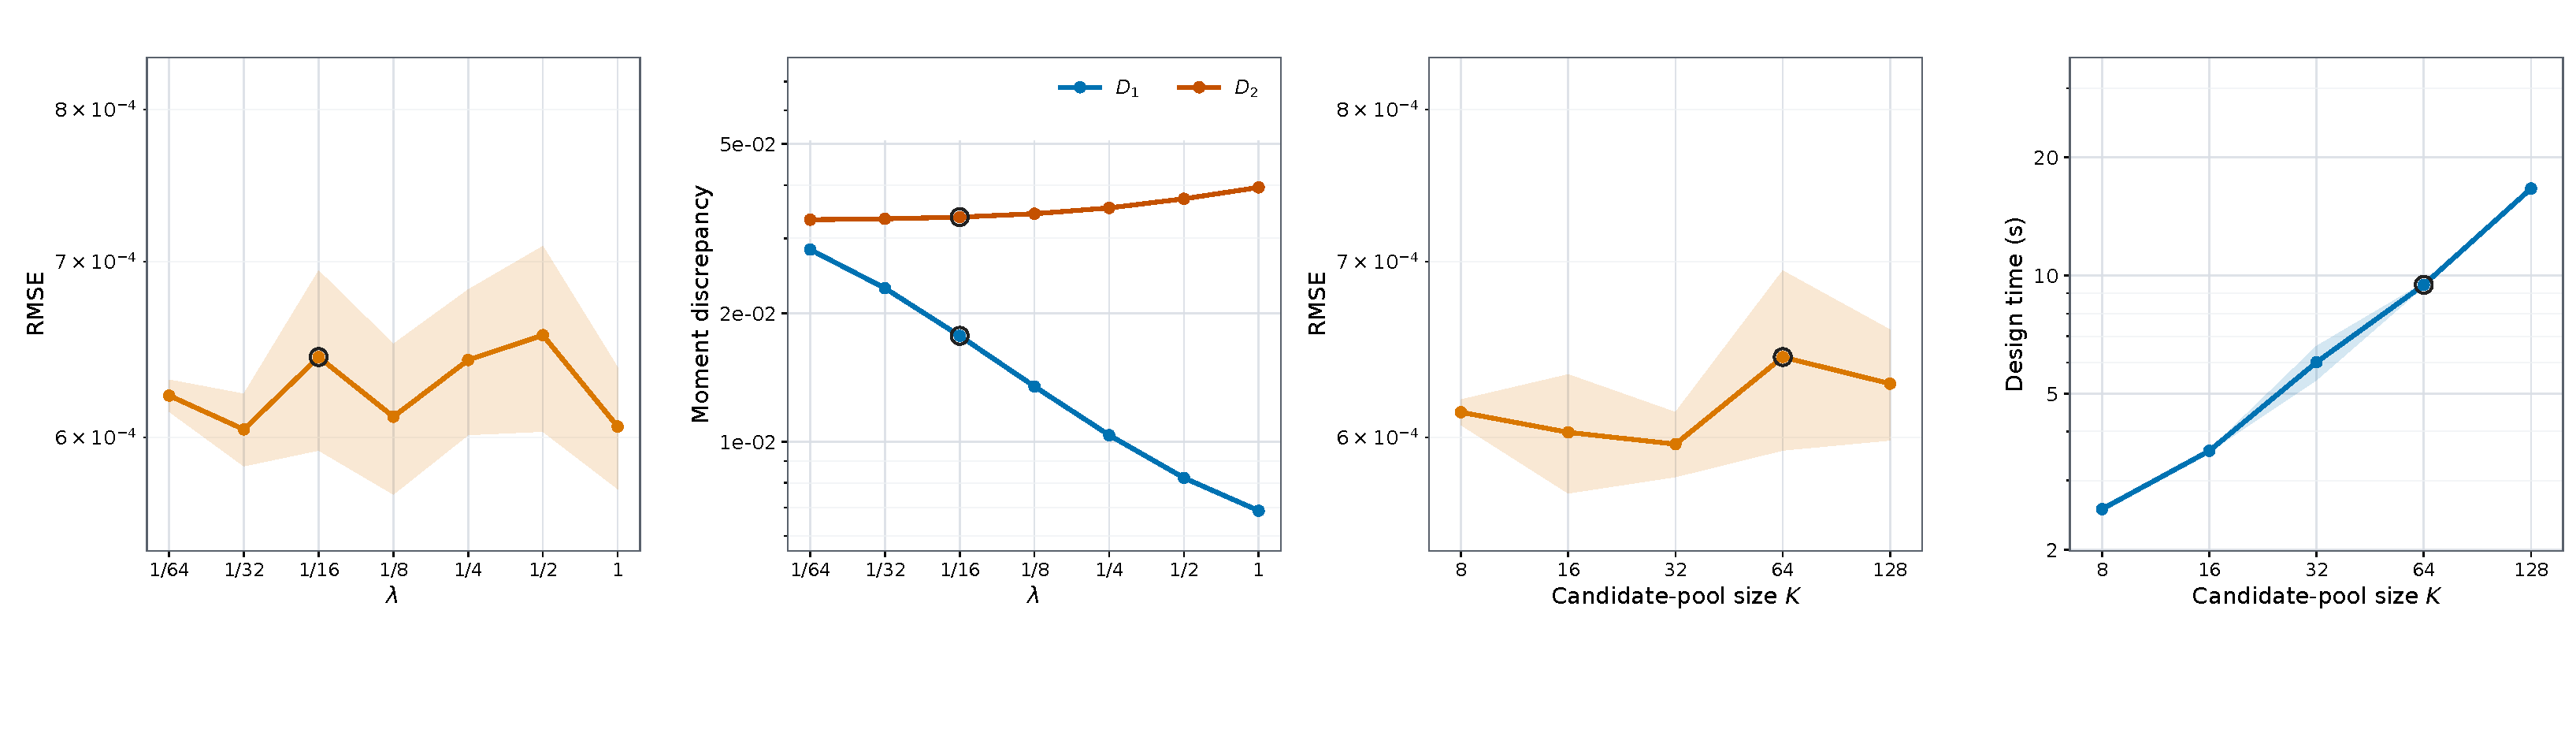
\includegraphics[width=\textwidth]{results/pdf/wine_inside_sensitivity.pdf}
\caption{Parameter sensitivity on Wine. From left to right: RMSE versus the normalized
weight $\lambda$ at $K=64$; equal-size moment discrepancies $D_1,D_2$
versus $\lambda$; RMSE versus $K$ at $\lambda=1/16$;
design-construction wall time versus $K$. Curves show means across three
paired estimator seeds; shading shows $\pm$ one sample standard deviation.
Black rings identify the pre-existing defaults. Axes are logarithmic;
the two RMSE panels share vertical limits. Design time uses 16 workers,
includes worker overhead, and excludes SVM evaluation and diagnostics.
Narrow standard-deviation bands can be hidden by the curve width.}
\label{fig:wine_sensitivity}
\end{figure}

On Breast Cancer, mean RMSE at $\lambda=1/32,1/16,1/8$ is respectively $0.0002351$, $0.0002367$, $0.0002402$; the largest is 2.1\% above the smallest. Moving from $K=64$ to $K=128$ changes mean RMSE from $0.0002367$ to $0.0002356$, while mean design time increases from 74.60 to 130.76 seconds.


\begin{figure}[t]
\centering
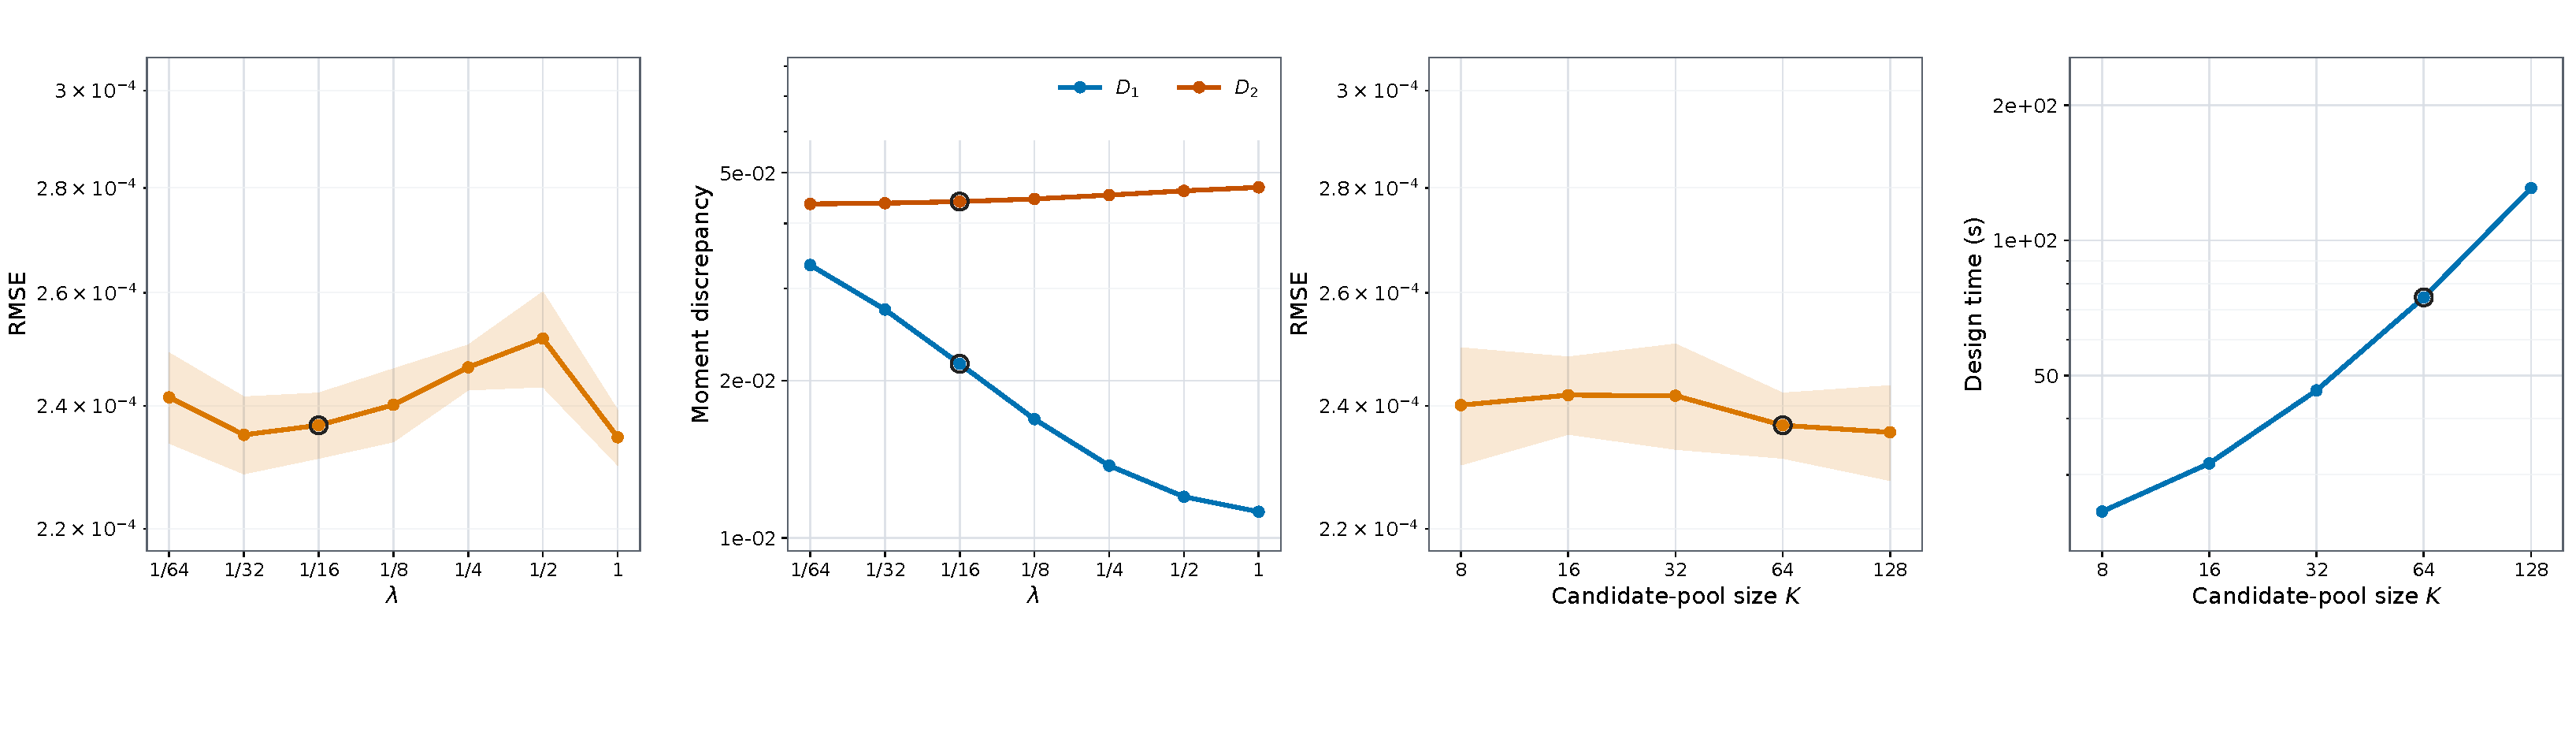
\includegraphics[width=\textwidth]{results/pdf/cancer_inside_sensitivity.pdf}
\caption{Parameter sensitivity on Breast Cancer. From left to right: RMSE versus the normalized
weight $\lambda$ at $K=64$; equal-size moment discrepancies $D_1,D_2$
versus $\lambda$; RMSE versus $K$ at $\lambda=1/16$;
design-construction wall time versus $K$. Curves show means across three
paired estimator seeds; shading shows $\pm$ one sample standard deviation.
Black rings identify the pre-existing defaults. Axes are logarithmic;
the two RMSE panels share vertical limits. Design time uses 16 workers,
includes worker overhead, and excludes SVM evaluation and diagnostics.
Narrow standard-deviation bands can be hidden by the curve width.}
\label{fig:cancer_sensitivity}
\end{figure}

These fixed-budget, three-repeat comparisons are descriptive; they do not establish statistical equivalence, a universal optimum, or accuracy saturation at $K=64$. The recorded Monte Carlo reference also has uncertainty, which is not included in the plotted seed standard deviations.
